\documentclass[landscape, headrule, footrule]{foils}
\usepackage{fancybox}
\usepackage[pdftex]{geometry}
\geometry{headsep= 0.2in, footskip=0.2in, hscale=0.9}

\usepackage[pdftex, usenames]{color}  %for colors
\usepackage[pdftex]{graphicx}     %for importing graphics
\usepackage{times}  %for nice fonts
\usepackage{background} 
\usepackage{pp4slide} 
\usepackage{pause} 
\usepackage{hyperref} %for hyperlinking and other 
                            %   pdf effects

\definecolor{DarkGreen}{rgb}{0.5,0.8,0.6}
\definecolor{RGBblack}{rgb}{0.0,0.0,0.0} 

%\vpagecolor[blue]{RGBblack} 

\hypersetup{
  pdftitle={Presentation using pdfLaTeX and \FoilTeX\, class},
  pdfsubject={How to make presentations with LaTeX},
  pdfauthor={Eugenia Yu and Weiliang Qiu,
    Department of Statistics,
    University of British Columbia},
  pdfkeywords={Presentations, LaTeX, FoilTeX, pdfTeX},
  pdfpagemode={FullScreen},                 %make the pdf start in full-screen
                                            %   mode
  %pdfpagemode={None},
  linkcolor=cyan,                           %make all the links cyan instead
  citecolor=cyan,                           %   of red
  pagecolor=cyan,
  urlcolor=cyan
  }

\leftheader{\textsc{Presentation using \textsc{pdf}\LaTeX\, and \FoilTeX\, class}}
                                            %make a left header
%\rightheader{\textsf{\thepage}}            %make a right header
\MyLogo{Eugenia and Weiliang, UBC Stats}    %make a left footer
%\rightfooter{}                             %make a right footer


\title{\shadowbox{Presentation using \textsc{pdf}\LaTeX\, and \FoilTeX\, class}} % the document title

% the author
\author{Latex Smart \\
         6356 Agricultural Road\\
         University of British Columbia\\
         Vancouver BC \\
         V6T 1Z2}

% the date
\date{\today}

\begin{document}

\thispagestyle{empty}

\setcounter{page}{0}

\maketitle

%\foilhead{}
%\LogoOn
%What does the term ``foil'' stand for?
%\vskip 2cm
%\begin{center}
%{\Large ?}
%\end{center}

\foilhead{Why use {\tt foils} class instead of {\tt seminar} class}
\LogoOn
\begin{itemize}
  \item nice centered titles and text in very large fonts\pause
  \item easy to rotate either the entire set of foils to landscape mode or to rotate individual
foils
  \item easy to control the header and footer
  \item directly produce {\tt pdf} output which can be displayed and printed in ``full-screen'' 
mode if combined with {\tt pdflatex}
\end{itemize}



\foilhead{Using \FoilTeX}
%\hypersetup{pdfpagetransition=Dissolve}

To create a simple presentation document using \FoilTeX, we
can use the \textcolor{red}{\tt foils} class. 
The syntax is as follows:

{\small
\begin{verbatim}
\documentclass[landscape]{foils}
...
\begin{document}
\foilhead[length]{title of page 1}
...
\foilhead[length]{title of next page}
...
\end{document}
\end{verbatim}
}
where the option {\tt length} specify the vertical space used as a cushion between the header
and the body of the foil. For example, if you want the body of your foil to sit closer to the
header, you could use the command
{\small
\begin{verbatim}
  \foilhead[-0.5in]{This is the Header}
\end{verbatim}
}

%\foilhead{Using \FoilTeX\, (ct'd)}
%\hypersetup{pdfpagetransition=Box}
%\FoilTeX \, is a document class for producing overhead projector slides
%and the like.  It is much simpler and prettier than \textsc{Sli}\TeX \,
%and the \texttt{seminar} class.

%Using \FoilTeX:
%\vspace{-0.2in}
%\begin{itemize}
%\item Declare the document class at the beginning of the document,
%  \verb|\documentclass[landscape]{foils}| and add
%  \verb|\usepackage{color}| in preamble for color slides.
%\item For each page \verb|\foilhead{This is the title of this slide}|.
%  \begin{itemize}
%    \item The \verb|\vspace| command is useful to get spacing right.
%    \item If there is too much text to fit on one slide, some will be put
%      on another slide (without a title).
%    \end{itemize}
%\end{itemize}

%That's it!

\rotatefoilhead{rotatefoilhead macros}

To rotate a foil, simply use \verb+\rotatefoilhead+ instead of
\verb+foilhead+

\begin{itemize}
  \item everything on the page will be rotate including header and footer.
  \item if the default position is portrait, then this foil will be rotated
to landscape.
  \item if the default position is landscape, then it rotates to portrait.
  \item if a rotated foil is splitted into several pages, then each of these
pages will also be rotated. Normal orientation is recovered by the next
invocation of \verb+\foilhead+.
\end{itemize}

\foilhead{Header and Footer}
\leftheader{left header $\Sigma$}
\rightheader{right header \thepage}
\rightfooter{right footer}

The code for this page's header and footer are
\begin{verbatim}
  \leftheader{left header $\Sigma$}
  \rightheader{right header \thepage}
  \rightfooter{right footer}
\end{verbatim}

To clear the header and footer, type
\begin{verbatim}
  \leftheader{}
  \rightheader{}
  \rightfooter{}
\end{verbatim}

To add ruler in the header and footer, use the {\tt headrule} and {\tt
footrule} class options.
{\small
\begin{verbatim}
\documentclass[landscape, headrule, footrule]{foils}
\end{verbatim}
}

\foilhead{Left Footer}

\leftheader{\textsc{Presentation using \textsc{pdf}\LaTeX\, and \FoilTeX\, class}}

\rightheader{}
\rightfooter{\thepage}
\MyLogo{This is my logo}
\Restriction{This is the content of my restriction}

\begin{itemize}
  \item The left footer is controlled by \verb+\MyLogo+ and \verb+\Restriction+
macro.

  \item By default, the footline consists of the contents of \verb+\MyLogo+
followed by the contents of \verb+\Restriction+.

  \item By default (\verb+\MyLogo{}+ and \verb+\Restriction{}+), \verb+\Restriction+ is empty and \verb+\MyLogo+ is the
phrase 

``-- Typeset by \FoilTeX\, --''.

  \item You can toggle on and off the logo by macro \verb+\LogoOn+ and
\verb+LogoOff+.
\end{itemize}


\foilhead{Installation of \FoilTeX and Compilation of Foil files}
\MyLogo{Eugenia and Weiliang, UBC Stats} 
\Restriction{}

We can download the \FoilTeX\, package from the following site:

\href{http://www.ctan.org/tex-archive/macros/latex/contrib/supported/foiltex/}{http://www.ctan.org/tex-archive/macros/latex/contrib/supported/foiltex/}

After downloading the necessary files, use command \verb1latex foiltex.ins1 for installation.

To compile a foil file, you can use command \verb+latex filename.tex+. It's
better to use command \verb+pdflatex filename.tex+.

\hyperlink{next page}{next page}

\foilhead{PDFLaTeX}

\hypertarget{next page}{}

\begin{itemize}
  \item PDFLaTex is a version of \LaTeX\, that generates PDF output
  \item PDF is a near-universal format
  \item PDF file can be ``full-screen'' displayed
  \item PDF has a number of advanced features --- special display effects,
hyperlinks, and so forth.
\end{itemize}

\foilhead[-0.5in]{Some Special Display Effects}
To make the pdf start in full-screen mode, use  
\begin{verbatim}
  \usepackage[pdftex]{geometry}
\end{verbatim}
 and use macro \verb+\hypersetup+. For
example,
\vskip -0.2cm
{\small
\begin{verbatim}
\hypersetup{
  pdftitle={Presentation using pdfLaTeX and \FoilTeX\, class},
  pdfsubject={How to make presentations with LaTeX},
  pdfauthor={Eugenia Yu and Weiliang Qiu,
    Department of Statistics,
    University of British Columbia},
  pdfkeywords={Presentations, LaTeX, FoilTeX, pdfTeX},
  pdfpagemode={FullScreen},   %make the pdf start in full-screen
                              %   mode
  linkcolor=cyan,             %make all the links cyan instead
  citecolor=cyan,             %   of red
  pagecolor=cyan,
  urlcolor=cyan
  }
\end{verbatim}
}

\foilhead[-0.5in]{Some Special Display Effects (Con't)}
\MyLogo{The content of this page is from: Hideo Umeki (2002),
{\it The geometry package}.}
%http://www.ctan.org/tex-archive/macros/latex/contrib/supported/geometry/manual.pdf}
\hypersetup{pdfpagetransition=Dissolve}
Effect of \verb+\hypersetup{pdfpagetransition=Dissolve}+

To set dimensions for page layout in \LaTeX\, is not straightforward. You
need to adjust several \LaTeX\, dimensions to place a text area where you
want. If you want to center the text area in the paper you use, for example,
you have to use specify \LaTeX\, dimensions as follows:
{\small
\begin{verbatim}
  \usepackage{calc}
  \setlength{\textwidth{8in}}
  \setlength{\textheight{11in}}
  \setlength\oddsidemargin{(\paperwidth-\textwidth)/2 - 1in}
  \setlength\topmargin{(\paperheight-\textheight
                        -headheight-\headsep-\footskip)/2 - 1in}
\end{verbatim}
}
Without {\tt calc} package, the above example would need more tedious
setting. The {\tt geometry} package provides an easy way to set page layout
parameters. In this case, what you have to do is just
{\small
\begin{verbatim}
  \usepackage[body={8in, 11in}]{geometry}.
\end{verbatim}
}

\foilhead[-0.5in]{Some Special Display Effects (Con't)}
\hypersetup{pdfpagetransition=Box}
Effect of  \verb+\hypersetup{pdfpagetransition=Box}+

The package ({\tt geometry}) will be also useful when you have to set page
layout obeying the following strict instructions: for example:
{\small
\begin{quote}
The total allowable width of the text area is 6.5 inches wide by 8.75 inches
high. The first line on each page should begin 1.2 inches from the top edge
of the page. The left margin should be 0.4 inch from the left edge.
\end{quote}
}
In this case, using {\tt geometry} package you can go
{\small
\begin{verbatim}
  \usepackage[body={6.5in, 8.75in},
                    top=1.2in, left=0.4in, nohead]{geometry}.
\end{verbatim}
}

\foilhead{}
\MyLogo{Eugenia and Weiliang, UBC Stats} 
\hypersetup{pdfpagetransition=Replace}

To switch off the {\tt pdfpagetransition}, use
\begin{verbatim}
\hypersetup{pdfpagetransition=Replace}
\end{verbatim}

\foilhead[-0.5in]{Hyperref Package}
\MyLogo{The content of this page is from: Sebastian Rahtz (1998),
{\it Hypertext marks in \LaTeX: the hyperref package}.}

\begin{itemize}
  \item The package {\tt hyperref} derives from, and builds on, 
the work of the HyperTEX project, described
at \verb+http://xxx.lanl.gov/hypertex/+. 
  \item It extends the functionality of all the LATEX
cross-referencing commands (including the table of contents, bibliographies 
etc).
  \item 
It also
provides new commands to allow the user to write ad hoc hypertext links, 
including
those to external documents and URLs.
\end{itemize}

\foilhead[-0.5in]{Hyperref Package (Con't)}
\MyLogo{Eugenia and Weiliang, UBC Stats} 
Syntax:
\begin{itemize}
  \item \verb+\href{URL}{text}+

Example: \verb+\href{http://www.stat.ubc.ca}{Stat Dept., UBC}+
$\Rightarrow$  \href{http://www.stat.ubc.ca}{Stat Dept., UBC}

  \item
\verb+\hyperlink{name}{text}+ and 
\verb+\hypertarget{name}{text}+

Example: \verb+\hyperlink{mycolor}{Color Package}+ $\Rightarrow$
\hyperlink{mycolor}{Color Package}. 

We define 
\verb+\hypertarget{mycolor}{Color Package}+ in the next page:
{\small
\begin{verbatim}
\foilhead[-0.5in]{\hypertarget{mycolor}{Color Package}}
\end{verbatim}
}
\end{itemize}

\foilhead[-0.5in]{\hypertarget{mycolor}{Color Package}}
\begin{itemize}
  \item \verb+\usepackage[usenames]{color}+

Here option {\tt [usenames]} causes the definitions for the $68$ colors
known to dvips to be preloaded. E.g. \verb+\textcolor{red}{red}+
produces \textcolor{red}{red}.
  \item You also can define your own custom colors. For example:
\verb+\definecolor{DarkGreen}{rgb}{0.5,0.8,0.6}+

\textcolor{DarkGreen}{This is DarkGreen}
  \item To add background color and other special dispaly effects of PDF
such as {\tt pause}, we can use {\tt ppower4}.
\end{itemize}


%\foilhead{Minipage and Graphics}
%\MyLogo{Eugenia and Weiliang, UBC Stats} 
%
%\begin{minipage}[t]{4.5in}
%  \raggedright
%  \begin{center}
%    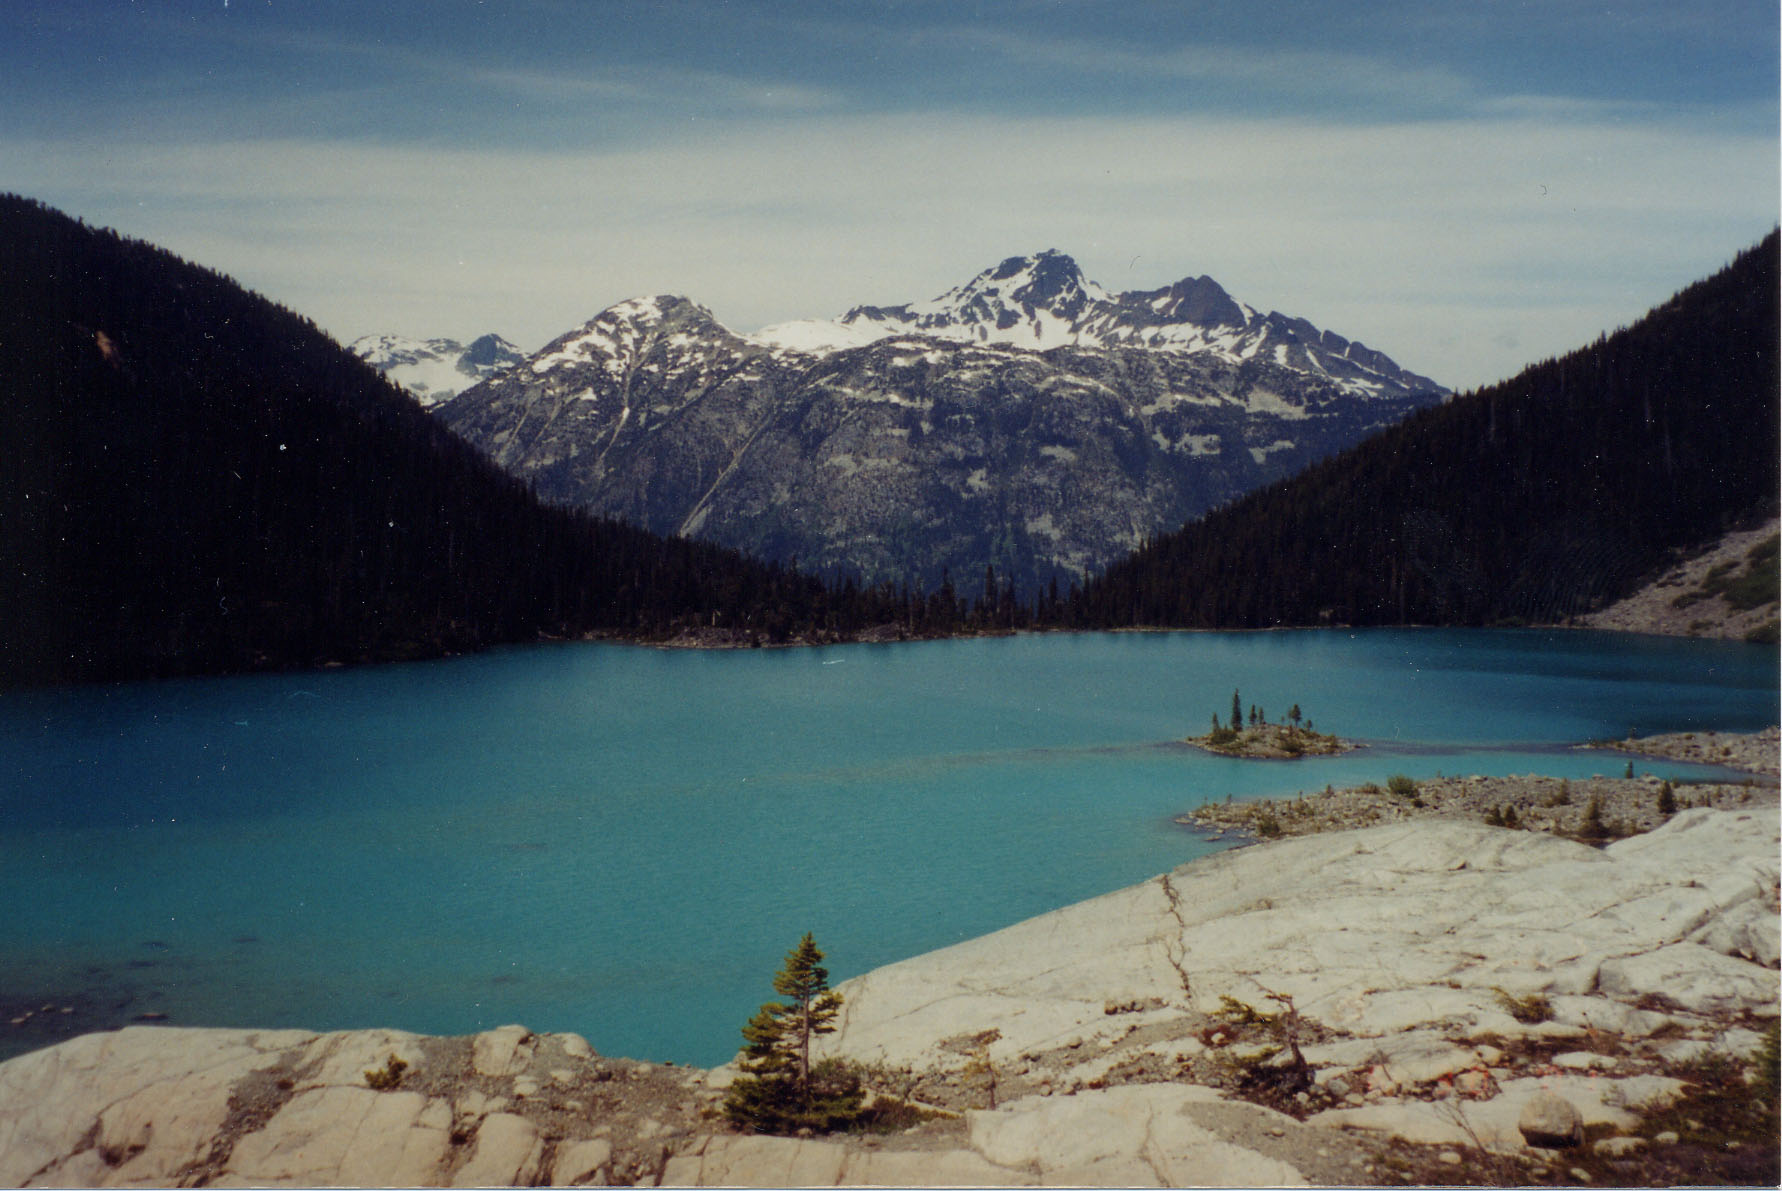
\includegraphics[width=2.8in,height=2in]{whistler}
%  \end{center}
%  \vspace{-0.2in}
%  \begin{itemize}
%  \item{\it Grad Trip}, August 2001
%  \vspace{-0.2in}
%    \begin{itemize}
%    \item Destination: Joffre Lake in Whistler 
%    \item People: UBC stats grads 
%    \item Activities: BBQ, hiking, canoeing, etc 
%  \end{itemize}
% \end{itemize}
%\end{minipage}
%\hfill
%\begin{minipage}[t]{4.5in}
%  \raggedright
%  \begin{center}
%    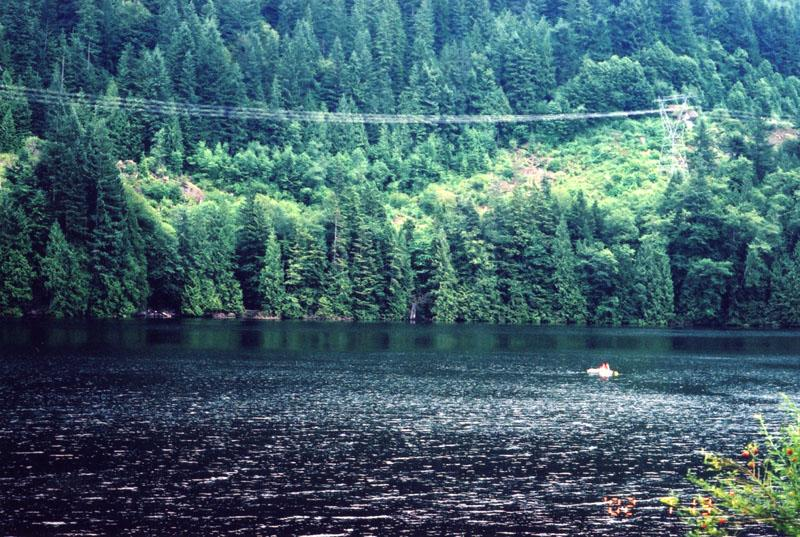
\includegraphics[width=2.8in,height=2in]{lake1}
%  \end{center}
%  \vspace{-0.2in}
%  \begin{itemize}
%  \item{\it Grad Trip}, July 2002
%  \vspace{-0.2in}
%    \begin{itemize}
%    \item Destination: Buntzen Lake in Port Coquitlam
%    \item People: UBC and SFU stats grads
%    \item Activities: BBQ, hiking, kayaking, etc
%    \end{itemize}
%  \end{itemize}
%\end{minipage}
%
\end{document}
